\documentclass[tikz]{standalone}

\usepackage{mathtools}

\let\Im\relax
\DeclareMathOperator{\Im}{Im}
\let\Re\relax
\DeclareMathOperator{\Re}{Re}

\usetikzlibrary{decorations.markings,positioning}

\providecommand{\poles}{
  \node (poles) at (2.5,1.5) {poles of $h(p_0)$};
  \draw[fill]
  (1.5,3) coordinate [circle,fill,inner sep=1pt,label=right:$p_1$] (p1)
  (2,-2) coordinate [circle,fill,inner sep=1pt,label=below:$p_2$] (p2)
  (-3,1) coordinate [circle,fill,inner sep=1pt,label=above:$p_3$] (p3)
  (-2,-1.5) coordinate [circle,fill,inner sep=1pt,label=above:$p_4$] (p4);
  \draw[ultra thin,gray] (poles) -- (p1) (poles) -- (p2) (poles.west) -- (p3) (poles) -- (p4);
}

\providecommand{\polecontours}{
  \draw[blue!60!black,decoration={markings,mark=between positions 0.03 and 1.03 step 0.125 with \arrow{<}},postaction={decorate}] (p1) circle (0.5) node [below=0.5] {$C_1$} (p2) circle (0.5) node [below=0.5] {$C_2$} (p3) circle (0.5) node [below=0.5] {$C_3$} (p4) circle (0.5) node [below=0.5] {$C_4$};
}

\begin{document}
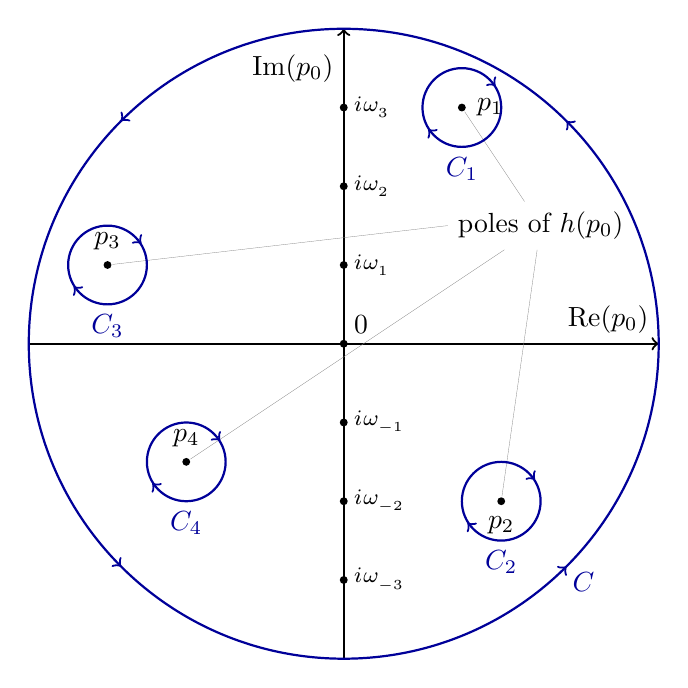
\begin{tikzpicture}[thick]

  \def\xr{3} \def\yr{3}

  % Axes
  \draw [->] (-\xr-1,0) -- (\xr+1,0) node [above left] {$\Re(p_0)$};
  \draw [->] (0,-\yr-1) -- (0,\yr+1) node [below left=0.2 and 0] {$\Im(p_0)$};

  % Matsubara frequencies
  \foreach \n in {-\yr,...,-1,1,2,...,\yr}{%
      \draw[fill] (0,\n) circle (1pt) node [right,font=\footnotesize] {$i \mkern1mu \omega_{_{\n}}$};}
  \draw[fill] (0,0) circle (1pt) node [above right] {0};

  % Contour line
  \draw[blue!60!black,decoration={markings,mark=between positions 0.125 and 0.875 step 0.25 with \arrow{>}},postaction={decorate}] circle (\yr+1) node [below right=0.925*\xr and 0.925*\yr] {$C$};

  % Poles
  \poles

  % Pole contours
  \polecontours

\end{tikzpicture}
\end{document}
